\documentclass[twoside]{book}

% Packages required by doxygen
\usepackage{fixltx2e}
\usepackage{calc}
\usepackage{doxygen}
\usepackage[export]{adjustbox} % also loads graphicx
\usepackage{graphicx}
\usepackage[utf8]{inputenc}
\usepackage{makeidx}
\usepackage{multicol}
\usepackage{multirow}
\PassOptionsToPackage{warn}{textcomp}
\usepackage{textcomp}
\usepackage[nointegrals]{wasysym}
\usepackage[table]{xcolor}

% Font selection
\usepackage[T1]{fontenc}
\usepackage[scaled=.90]{helvet}
\usepackage{courier}
\usepackage{amssymb}
\usepackage{sectsty}
\renewcommand{\familydefault}{\sfdefault}
\allsectionsfont{%
  \fontseries{bc}\selectfont%
  \color{darkgray}%
}
\renewcommand{\DoxyLabelFont}{%
  \fontseries{bc}\selectfont%
  \color{darkgray}%
}
\newcommand{\+}{\discretionary{\mbox{\scriptsize$\hookleftarrow$}}{}{}}

% Page & text layout
\usepackage{geometry}
\geometry{%
  a4paper,%
  top=2.5cm,%
  bottom=2.5cm,%
  left=2.5cm,%
  right=2.5cm%
}
\tolerance=750
\hfuzz=15pt
\hbadness=750
\setlength{\emergencystretch}{15pt}
\setlength{\parindent}{0cm}
\setlength{\parskip}{3ex plus 2ex minus 2ex}
\makeatletter
\renewcommand{\paragraph}{%
  \@startsection{paragraph}{4}{0ex}{-1.0ex}{1.0ex}{%
    \normalfont\normalsize\bfseries\SS@parafont%
  }%
}
\renewcommand{\subparagraph}{%
  \@startsection{subparagraph}{5}{0ex}{-1.0ex}{1.0ex}{%
    \normalfont\normalsize\bfseries\SS@subparafont%
  }%
}
\makeatother

% Headers & footers
\usepackage{fancyhdr}
\pagestyle{fancyplain}
\fancyhead[LE]{\fancyplain{}{\bfseries\thepage}}
\fancyhead[CE]{\fancyplain{}{}}
\fancyhead[RE]{\fancyplain{}{\bfseries\leftmark}}
\fancyhead[LO]{\fancyplain{}{\bfseries\rightmark}}
\fancyhead[CO]{\fancyplain{}{}}
\fancyhead[RO]{\fancyplain{}{\bfseries\thepage}}
\fancyfoot[LE]{\fancyplain{}{}}
\fancyfoot[CE]{\fancyplain{}{}}
\fancyfoot[RE]{\fancyplain{}{\bfseries\scriptsize Generated by Doxygen }}
\fancyfoot[LO]{\fancyplain{}{\bfseries\scriptsize Generated by Doxygen }}
\fancyfoot[CO]{\fancyplain{}{}}
\fancyfoot[RO]{\fancyplain{}{}}
\renewcommand{\footrulewidth}{0.4pt}
\renewcommand{\chaptermark}[1]{%
  \markboth{#1}{}%
}
\renewcommand{\sectionmark}[1]{%
  \markright{\thesection\ #1}%
}

% Indices & bibliography
\usepackage{natbib}
\usepackage[titles]{tocloft}
\setcounter{tocdepth}{3}
\setcounter{secnumdepth}{5}
\makeindex

% Hyperlinks (required, but should be loaded last)
\usepackage{ifpdf}
\ifpdf
  \usepackage[pdftex,pagebackref=true]{hyperref}
\else
  \usepackage[ps2pdf,pagebackref=true]{hyperref}
\fi
\hypersetup{%
  colorlinks=true,%
  linkcolor=blue,%
  citecolor=blue,%
  unicode%
}

% Custom commands
\newcommand{\clearemptydoublepage}{%
  \newpage{\pagestyle{empty}\cleardoublepage}%
}

\usepackage{caption}
\captionsetup{labelsep=space,justification=centering,font={bf},singlelinecheck=off,skip=4pt,position=top}

%===== C O N T E N T S =====

\begin{document}

% Titlepage & ToC
\hypersetup{pageanchor=false,
             bookmarksnumbered=true,
             pdfencoding=unicode
            }
\pagenumbering{alph}
\begin{titlepage}
\vspace*{7cm}
\begin{center}%
{\Large My Project }\\
\vspace*{1cm}
{\large Generated by Doxygen 1.8.12}\\
\end{center}
\end{titlepage}
\clearemptydoublepage
\pagenumbering{roman}
\tableofcontents
\clearemptydoublepage
\pagenumbering{arabic}
\hypersetup{pageanchor=true}

%--- Begin generated contents ---
\chapter{Hierarchical Index}
\section{Class Hierarchy}
This inheritance list is sorted roughly, but not completely, alphabetically\+:\begin{DoxyCompactList}
\item \contentsline{section}{character\+:\+:abil\+List}{\pageref{structcharacter_1_1abil_list}}{}
\item basic\+\_\+streambuf\begin{DoxyCompactList}
\item \contentsline{section}{Q\+\_\+\+Debug\+Stream}{\pageref{class_q___debug_stream}}{}
\item \contentsline{section}{Q\+\_\+\+Debug\+Stream}{\pageref{class_q___debug_stream}}{}
\end{DoxyCompactList}
\item \contentsline{section}{character}{\pageref{classcharacter}}{}
\item \contentsline{section}{item\+Container}{\pageref{classitem_container}}{}
\item \contentsline{section}{Map\+Screen}{\pageref{class_map_screen}}{}
\item \contentsline{section}{observer}{\pageref{classobserver}}{}
\begin{DoxyCompactList}
\item \contentsline{section}{character\+Observer}{\pageref{classcharacter_observer}}{}
\end{DoxyCompactList}
\item Q\+Graphics\+Scene\begin{DoxyCompactList}
\item \contentsline{section}{Grid\+Scene}{\pageref{class_grid_scene}}{}
\end{DoxyCompactList}
\item Q\+Main\+Window\begin{DoxyCompactList}
\item \contentsline{section}{character\+Observer}{\pageref{classcharacter_observer}}{}
\item \contentsline{section}{editscreen}{\pageref{classeditscreen}}{}
\item \contentsline{section}{test\+Qt}{\pageref{classtest_qt}}{}
\end{DoxyCompactList}
\item Q\+Object\begin{DoxyCompactList}
\item \contentsline{section}{character\+Controller}{\pageref{classcharacter_controller}}{}
\end{DoxyCompactList}
\item Q\+Widget\begin{DoxyCompactList}
\item \contentsline{section}{logic}{\pageref{classlogic}}{}
\end{DoxyCompactList}
\item \contentsline{section}{Search}{\pageref{struct_search}}{}
\item \contentsline{section}{Space}{\pageref{struct_space}}{}
\item Test\+Fixture\begin{DoxyCompactList}
\item \contentsline{section}{character\+Test}{\pageref{classcharacter_test}}{}
\end{DoxyCompactList}
\end{DoxyCompactList}

\chapter{Class Index}
\section{Class List}
Here are the classes, structs, unions and interfaces with brief descriptions\+:\begin{DoxyCompactList}
\item\contentsline{section}{\hyperlink{structcharacter_1_1abil_list}{character\+::abil\+List} }{\pageref{structcharacter_1_1abil_list}}{}
\item\contentsline{section}{\hyperlink{classcharacter}{character} }{\pageref{classcharacter}}{}
\item\contentsline{section}{\hyperlink{classcharacter_controller}{character\+Controller} }{\pageref{classcharacter_controller}}{}
\item\contentsline{section}{\hyperlink{classcharacter_observer}{character\+Observer} }{\pageref{classcharacter_observer}}{}
\item\contentsline{section}{\hyperlink{classcharacter_test}{character\+Test} }{\pageref{classcharacter_test}}{}
\item\contentsline{section}{\hyperlink{classeditscreen}{editscreen} }{\pageref{classeditscreen}}{}
\item\contentsline{section}{\hyperlink{class_grid_scene}{Grid\+Scene} }{\pageref{class_grid_scene}}{}
\item\contentsline{section}{\hyperlink{classitem_container}{item\+Container} }{\pageref{classitem_container}}{}
\item\contentsline{section}{\hyperlink{classlogic}{logic} }{\pageref{classlogic}}{}
\item\contentsline{section}{\hyperlink{class_map_screen}{Map\+Screen} }{\pageref{class_map_screen}}{}
\item\contentsline{section}{\hyperlink{classobserver}{observer} }{\pageref{classobserver}}{}
\item\contentsline{section}{\hyperlink{class_q___debug_stream}{Q\+\_\+\+Debug\+Stream} }{\pageref{class_q___debug_stream}}{}
\item\contentsline{section}{\hyperlink{struct_search}{Search} }{\pageref{struct_search}}{}
\item\contentsline{section}{\hyperlink{struct_space}{Space} }{\pageref{struct_space}}{}
\item\contentsline{section}{\hyperlink{classtest_qt}{test\+Qt} }{\pageref{classtest_qt}}{}
\end{DoxyCompactList}

\chapter{Class Documentation}
\hypertarget{structcharacter_1_1abil_list}{}\section{character\+:\+:abil\+List Struct Reference}
\label{structcharacter_1_1abil_list}\index{character\+::abil\+List@{character\+::abil\+List}}
\subsection*{Public Attributes}
\begin{DoxyCompactItemize}
\item 
\hypertarget{structcharacter_1_1abil_list_a47b62372951fd49c02cde454fdc54af3}{}\label{structcharacter_1_1abil_list_a47b62372951fd49c02cde454fdc54af3} 
int {\bfseries strength}
\item 
\hypertarget{structcharacter_1_1abil_list_a39aa5b2ebf613f1c16698b115fc8d94b}{}\label{structcharacter_1_1abil_list_a39aa5b2ebf613f1c16698b115fc8d94b} 
int {\bfseries intelligence}
\item 
\hypertarget{structcharacter_1_1abil_list_a5b7b5c1a7de429425cae26e56f7af95e}{}\label{structcharacter_1_1abil_list_a5b7b5c1a7de429425cae26e56f7af95e} 
int {\bfseries wisdom}
\item 
\hypertarget{structcharacter_1_1abil_list_aac36eb9c4f417f95004d000d88d763c4}{}\label{structcharacter_1_1abil_list_aac36eb9c4f417f95004d000d88d763c4} 
int {\bfseries dexterity}
\item 
\hypertarget{structcharacter_1_1abil_list_a96f3881abe36ac9cd08ea164c6078feb}{}\label{structcharacter_1_1abil_list_a96f3881abe36ac9cd08ea164c6078feb} 
int {\bfseries constitution}
\item 
\hypertarget{structcharacter_1_1abil_list_a19859232e9c642604134f73c61c3c797}{}\label{structcharacter_1_1abil_list_a19859232e9c642604134f73c61c3c797} 
int {\bfseries charisma}
\end{DoxyCompactItemize}


The documentation for this struct was generated from the following file\+:\begin{DoxyCompactItemize}
\item 
test\+Qt/character.\+h\end{DoxyCompactItemize}

\hypertarget{classcharacter}{}\section{character Class Reference}
\label{classcharacter}\index{character@{character}}


{\ttfamily \#include $<$character.\+h$>$}

\subsection*{Classes}
\begin{DoxyCompactItemize}
\item 
struct \hyperlink{structcharacter_1_1abil_list}{abil\+List}
\end{DoxyCompactItemize}
\subsection*{Public Member Functions}
\begin{DoxyCompactItemize}
\item 
\hypertarget{classcharacter_a7f19c0ee3b827b017eff3ad6fae5c422}{}\label{classcharacter_a7f19c0ee3b827b017eff3ad6fae5c422} 
{\bfseries character} (int i, std\+::string n, int l, std\+::string im)
\item 
\hypertarget{classcharacter_adeb8d2beadcc402ce388606cdaa0bba6}{}\label{classcharacter_adeb8d2beadcc402ce388606cdaa0bba6} 
{\bfseries character} (int i, std\+::string n, int l, std\+::string im, int abilities\mbox{[}6\mbox{]})
\item 
\hypertarget{classcharacter_a8dcd236fcff892e4515e859318072551}{}\label{classcharacter_a8dcd236fcff892e4515e859318072551} 
void {\bfseries set\+Id} (int i)
\item 
\hypertarget{classcharacter_ae9dffcbabcac5371a92f442a08b497fd}{}\label{classcharacter_ae9dffcbabcac5371a92f442a08b497fd} 
void {\bfseries set\+Name} (std\+::string n)
\item 
\hypertarget{classcharacter_a1debcb88c0662f8b361122b4261d777c}{}\label{classcharacter_a1debcb88c0662f8b361122b4261d777c} 
void {\bfseries set\+Level} (int l)
\item 
\hypertarget{classcharacter_a528b7881f18a272cd71bb4f442c5ad80}{}\label{classcharacter_a528b7881f18a272cd71bb4f442c5ad80} 
void {\bfseries set\+HP} (int hp)
\item 
\hypertarget{classcharacter_ae25486dd054cd4c9202111b616794a8e}{}\label{classcharacter_ae25486dd054cd4c9202111b616794a8e} 
void {\bfseries dec\+HP} (int damage)
\item 
\hypertarget{classcharacter_a342bf66b25c7f8e5b006ed88a85c7183}{}\label{classcharacter_a342bf66b25c7f8e5b006ed88a85c7183} 
int {\bfseries get\+Armor\+Bonus} ()
\item 
\hypertarget{classcharacter_aa9641ce584c23e39fa9a085afa1b8d5b}{}\label{classcharacter_aa9641ce584c23e39fa9a085afa1b8d5b} 
virtual int {\bfseries get\+Damage\+Bonus} ()
\item 
\hypertarget{classcharacter_a926466b75c8655ca69385780ad3f1a0b}{}\label{classcharacter_a926466b75c8655ca69385780ad3f1a0b} 
virtual int {\bfseries get\+Attack\+Bonus} ()
\item 
int \hyperlink{classcharacter_a7545a786510f968f6299e8975e6b6b06}{get\+Max\+HP} ()
\item 
\hypertarget{classcharacter_aae5fa02f62b32f9daa389d8d68d5b4d6}{}\label{classcharacter_aae5fa02f62b32f9daa389d8d68d5b4d6} 
void {\bfseries set\+Image} (std\+::string im)
\item 
\hypertarget{classcharacter_a67c8168cb18f99febc2e4160a8e0c58c}{}\label{classcharacter_a67c8168cb18f99febc2e4160a8e0c58c} 
void {\bfseries setX} (int x)
\item 
\hypertarget{classcharacter_a1161fcef69fd85b3e2dcf9ff20b9b471}{}\label{classcharacter_a1161fcef69fd85b3e2dcf9ff20b9b471} 
void {\bfseries setY} (int y)
\item 
\hypertarget{classcharacter_a153c1d1989f5cb13e9ddcf8881f74701}{}\label{classcharacter_a153c1d1989f5cb13e9ddcf8881f74701} 
void {\bfseries move\+By} (int x, int y)
\item 
\hypertarget{classcharacter_a6af93dc6977752b5e91bda0b2a28841a}{}\label{classcharacter_a6af93dc6977752b5e91bda0b2a28841a} 
void {\bfseries move\+To} (int x, int y)
\item 
\hypertarget{classcharacter_a081aaac1bcb0854c6579710746ca3c71}{}\label{classcharacter_a081aaac1bcb0854c6579710746ca3c71} 
virtual int {\bfseries get\+HP} ()
\item 
\hypertarget{classcharacter_a242a91b319a57b29c4014937bedd4e37}{}\label{classcharacter_a242a91b319a57b29c4014937bedd4e37} 
int {\bfseries get\+Id} ()
\item 
\hypertarget{classcharacter_ac2afed052f62a7eb2bf181d2f2258fd1}{}\label{classcharacter_ac2afed052f62a7eb2bf181d2f2258fd1} 
std\+::string {\bfseries get\+Name} ()
\item 
\hypertarget{classcharacter_a185635ea352e657170ab839a491a47f5}{}\label{classcharacter_a185635ea352e657170ab839a491a47f5} 
int {\bfseries get\+Level} ()
\item 
\hypertarget{classcharacter_ab65accb5f45aa00aec892e71ec292174}{}\label{classcharacter_ab65accb5f45aa00aec892e71ec292174} 
\hyperlink{structcharacter_1_1abil_list}{character\+::abil\+List} {\bfseries get\+Abilities} ()
\item 
\hypertarget{classcharacter_ac2f4739d203695f4eda1536dca5fcfed}{}\label{classcharacter_ac2f4739d203695f4eda1536dca5fcfed} 
std\+::string {\bfseries get\+Class\+Name} ()
\item 
\hypertarget{classcharacter_a18dce66a2f2431a60e5a8e8c970aff44}{}\label{classcharacter_a18dce66a2f2431a60e5a8e8c970aff44} 
virtual int {\bfseries level\+Up} (int inc\+Amount)
\item 
\hypertarget{classcharacter_a76a4dede3755507ba76953080d4c729c}{}\label{classcharacter_a76a4dede3755507ba76953080d4c729c} 
std\+::string {\bfseries get\+Image} ()
\item 
\hypertarget{classcharacter_a5a8739169623487c1d2a7626b37e2886}{}\label{classcharacter_a5a8739169623487c1d2a7626b37e2886} 
int {\bfseries getX} ()
\item 
\hypertarget{classcharacter_a9ac85ca2d1a1930ef4ecf069997be39f}{}\label{classcharacter_a9ac85ca2d1a1930ef4ecf069997be39f} 
int {\bfseries getY} ()
\item 
\hypertarget{classcharacter_a14a67dba3fa314ce52f23966fa55bd22}{}\label{classcharacter_a14a67dba3fa314ce52f23966fa55bd22} 
\hyperlink{structcharacter_1_1abil_list}{abil\+List} {\bfseries generate\+Abilities} ()
\item 
\hypertarget{classcharacter_ae4482570a73550e4de68a5088e4166fa}{}\label{classcharacter_ae4482570a73550e4de68a5088e4166fa} 
int {\bfseries roll\+Dice} (int faces)
\item 
\hypertarget{classcharacter_a79782f747741ca665c4002969cccb1a1}{}\label{classcharacter_a79782f747741ca665c4002969cccb1a1} 
int {\bfseries get\+Max\+Roll\+Sum} (int faces, int num\+Rolls)
\item 
\hypertarget{classcharacter_a31b1482c77e8e8e81791ff6c6b83f334}{}\label{classcharacter_a31b1482c77e8e8e81791ff6c6b83f334} 
void {\bfseries add\+Observer} (\hyperlink{classobserver}{observer} \&obs)
\item 
\hypertarget{classcharacter_a8457474b31e7f3e8b3a3c48d5f564b96}{}\label{classcharacter_a8457474b31e7f3e8b3a3c48d5f564b96} 
void {\bfseries remove\+Observer} (\hyperlink{classobserver}{observer} \&obs)
\item 
\hypertarget{classcharacter_aaf06669f3ed8751518bad227f7a3cf11}{}\label{classcharacter_aaf06669f3ed8751518bad227f7a3cf11} 
bool {\bfseries is\+Attached} (\hyperlink{classobserver}{observer} $\ast$obs)
\item 
\hypertarget{classcharacter_ae514d5a8a08ac6437eb425d7d1ecd9d2}{}\label{classcharacter_ae514d5a8a08ac6437eb425d7d1ecd9d2} 
void {\bfseries notify\+Observers} ()
\end{DoxyCompactItemize}
\subsection*{Static Public Member Functions}
\begin{DoxyCompactItemize}
\item 
\hypertarget{classcharacter_a2551d2c84e185b12dabfdb4746af3519}{}\label{classcharacter_a2551d2c84e185b12dabfdb4746af3519} 
static int {\bfseries get\+Modifier} (int ability\+Score)
\end{DoxyCompactItemize}


\subsection{Detailed Description}
Character class. Contains all information related to a character. For the time being, the only character class is fighter. A character can be linked to an image file, which will be used to display him on the map.

DnD Rules\+: -\/\+Level\+: For the level, we use a maximum level of 20. This level is first set at character creation, but can afterwards be increased.

-\/\+Abilities\+: There are six different abilities, represented by a struct, and which can be set by the player of generated randomly. If generated randomly, each ability will be given by rolling a 6-\/dice four times and taking the sum of the 3 highest throws.

-\/\+Ability modifiers\+: Ability modifiers are given by the formula (ability level-\/10)/2

-\/\+HP\+: HP upon character creation is defined by the formula\+: (Hit Dice)+(Character Level)$\ast$(Constitution modifier). Afterwards, the HP can be increased or decreased, when a character heals or is injured. When a character levels up, his HP is increased by an amount equal to his constitution modifier.

-\/\+Hit Dice\+: fighters have a hit dice of 10, which represents some sort of value related to their ability to survive, I suppose.

-\/\+Armor Bonus\+: Armor bonus is the sum of\+: 10+(armor bonus)+(shield bonus)+(dexterity modifier)

-\/\+Attack Bonus\+: Attack bonus is given by\+: proficiency bonus (see below) plus a modifier (strenght if short range weapon, dexterity if long range) plus a dice roll of the weapon\textquotesingle{}s dice.

Design\+: The character class keeps a set of observers. When the character\textquotesingle{}s state changes, the observers are notified. Std\+::set was used to keep the set of observers, because it doesn\textquotesingle{}t allow for duplicates and generally corresponds to our needs. 

\subsection{Member Function Documentation}
\hypertarget{classcharacter_a7545a786510f968f6299e8975e6b6b06}{}\label{classcharacter_a7545a786510f968f6299e8975e6b6b06} 
\index{character@{character}!get\+Max\+HP@{get\+Max\+HP}}
\index{get\+Max\+HP@{get\+Max\+HP}!character@{character}}
\subsubsection{\texorpdfstring{get\+Max\+H\+P()}{getMaxHP()}}
{\footnotesize\ttfamily int character\+::get\+Max\+HP (\begin{DoxyParamCaption}{ }\end{DoxyParamCaption})}

returns the maximum starting HP for the character\textquotesingle{}s level, class and constitution 

The documentation for this class was generated from the following files\+:\begin{DoxyCompactItemize}
\item 
test\+Qt/character.\+h\item 
test\+Qt/character.\+cpp\end{DoxyCompactItemize}

\hypertarget{classcharacter_controller}{}\section{character\+Controller Class Reference}
\label{classcharacter_controller}\index{character\+Controller@{character\+Controller}}


{\ttfamily \#include $<$character\+Controller.\+h$>$}

Inheritance diagram for character\+Controller\+:\begin{figure}[H]
\begin{center}
\leavevmode
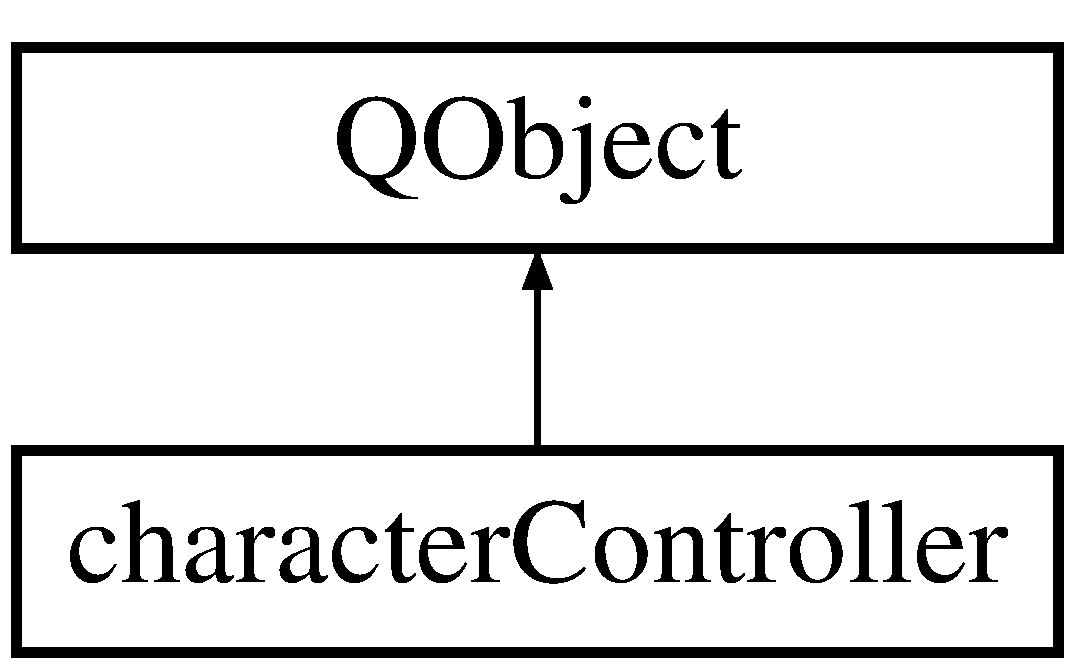
\includegraphics[height=2.000000cm]{classcharacter_controller}
\end{center}
\end{figure}
\subsection*{Public Slots}
\begin{DoxyCompactItemize}
\item 
void \hyperlink{classcharacter_controller_a4a3fa0e57a91c304be2adc2240041441}{set\+Character\+Name} ()
\item 
void \hyperlink{classcharacter_controller_a70eba4e82bdb8795f21a96be2f742fa0}{level\+Up\+Character} ()
\end{DoxyCompactItemize}
\subsection*{Public Member Functions}
\begin{DoxyCompactItemize}
\item 
\hypertarget{classcharacter_controller_aa49479f3b344083a024b94058f90c2cd}{}\label{classcharacter_controller_aa49479f3b344083a024b94058f90c2cd} 
{\bfseries character\+Controller} (\hyperlink{classcharacter}{character} $\ast$mod)
\end{DoxyCompactItemize}


\subsection{Detailed Description}
This class allows modification of the character class, so as to demonstrate the behavior of the \hyperlink{classcharacter_observer}{character\+Observer} class. 

\subsection{Member Function Documentation}
\hypertarget{classcharacter_controller_a70eba4e82bdb8795f21a96be2f742fa0}{}\label{classcharacter_controller_a70eba4e82bdb8795f21a96be2f742fa0} 
\index{character\+Controller@{character\+Controller}!level\+Up\+Character@{level\+Up\+Character}}
\index{level\+Up\+Character@{level\+Up\+Character}!character\+Controller@{character\+Controller}}
\subsubsection{\texorpdfstring{level\+Up\+Character}{levelUpCharacter}}
{\footnotesize\ttfamily void character\+Controller\+::level\+Up\+Character (\begin{DoxyParamCaption}{ }\end{DoxyParamCaption})\hspace{0.3cm}{\ttfamily [slot]}}

Increases the character level \hypertarget{classcharacter_controller_a4a3fa0e57a91c304be2adc2240041441}{}\label{classcharacter_controller_a4a3fa0e57a91c304be2adc2240041441} 
\index{character\+Controller@{character\+Controller}!set\+Character\+Name@{set\+Character\+Name}}
\index{set\+Character\+Name@{set\+Character\+Name}!character\+Controller@{character\+Controller}}
\subsubsection{\texorpdfstring{set\+Character\+Name}{setCharacterName}}
{\footnotesize\ttfamily void character\+Controller\+::set\+Character\+Name (\begin{DoxyParamCaption}{ }\end{DoxyParamCaption})\hspace{0.3cm}{\ttfamily [slot]}}

Sets the character name to a predefined value 

The documentation for this class was generated from the following files\+:\begin{DoxyCompactItemize}
\item 
test\+Qt/character\+Controller.\+h\item 
test\+Qt/character\+Controller.\+cpp\end{DoxyCompactItemize}

\hypertarget{classcharacter_observer}{}\section{character\+Observer Class Reference}
\label{classcharacter_observer}\index{character\+Observer@{character\+Observer}}


{\ttfamily \#include $<$character\+Observer.\+h$>$}

Inheritance diagram for character\+Observer\+:\begin{figure}[H]
\begin{center}
\leavevmode
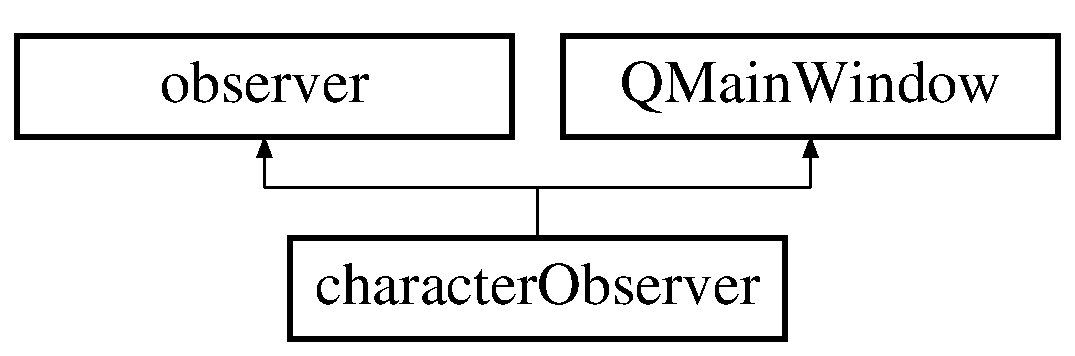
\includegraphics[height=2.000000cm]{classcharacter_observer}
\end{center}
\end{figure}
\subsection*{Public Member Functions}
\begin{DoxyCompactItemize}
\item 
\hypertarget{classcharacter_observer_a076a0222ae36d51b761298ed5ae3ec71}{}\label{classcharacter_observer_a076a0222ae36d51b761298ed5ae3ec71} 
{\bfseries character\+Observer} (Q\+Widget $\ast$parent, \hyperlink{classcharacter}{character} $\ast$sub)
\item 
void \hyperlink{classcharacter_observer_acef1a20aefd63499e3cbcad9fdfd7e02}{notify} ()
\item 
void \hyperlink{classcharacter_observer_a617083ec4e753ede947c6a355df18dfe}{initialize} ()
\item 
void \hyperlink{classcharacter_observer_a1a3ec8b3be1a73dc89e413dc817a6077}{update\+Table} ()
\end{DoxyCompactItemize}


\subsection{Detailed Description}
Character observer class, implementing the observer pattern. It also inherits the Q\+Main\+Window class of the QT framework. This class generates a QT table widget, where the character\textquotesingle{}s stats are displayed. In the final application, this will be used by the player to monitor his character\textquotesingle{}s or the npc\textquotesingle{}s stats.

The QT framework was chosen because of its simplicity and good documentation 

\subsection{Member Function Documentation}
\hypertarget{classcharacter_observer_a617083ec4e753ede947c6a355df18dfe}{}\label{classcharacter_observer_a617083ec4e753ede947c6a355df18dfe} 
\index{character\+Observer@{character\+Observer}!initialize@{initialize}}
\index{initialize@{initialize}!character\+Observer@{character\+Observer}}
\subsubsection{\texorpdfstring{initialize()}{initialize()}}
{\footnotesize\ttfamily void character\+Observer\+::initialize (\begin{DoxyParamCaption}{ }\end{DoxyParamCaption})}

Initializes the table displaying the character\textquotesingle{}s stats \hypertarget{classcharacter_observer_acef1a20aefd63499e3cbcad9fdfd7e02}{}\label{classcharacter_observer_acef1a20aefd63499e3cbcad9fdfd7e02} 
\index{character\+Observer@{character\+Observer}!notify@{notify}}
\index{notify@{notify}!character\+Observer@{character\+Observer}}
\subsubsection{\texorpdfstring{notify()}{notify()}}
{\footnotesize\ttfamily void character\+Observer\+::notify (\begin{DoxyParamCaption}{ }\end{DoxyParamCaption})\hspace{0.3cm}{\ttfamily [virtual]}}

Notifies the observer of a state change in the subject, prompting it to update its display 

Implements \hyperlink{classobserver}{observer}.

\hypertarget{classcharacter_observer_a1a3ec8b3be1a73dc89e413dc817a6077}{}\label{classcharacter_observer_a1a3ec8b3be1a73dc89e413dc817a6077} 
\index{character\+Observer@{character\+Observer}!update\+Table@{update\+Table}}
\index{update\+Table@{update\+Table}!character\+Observer@{character\+Observer}}
\subsubsection{\texorpdfstring{update\+Table()}{updateTable()}}
{\footnotesize\ttfamily void character\+Observer\+::update\+Table (\begin{DoxyParamCaption}{ }\end{DoxyParamCaption})}

Updates the table with the new character\textquotesingle{}s stats 

The documentation for this class was generated from the following files\+:\begin{DoxyCompactItemize}
\item 
test\+Qt/character\+Observer.\+h\item 
test\+Qt/character\+Observer.\+cpp\end{DoxyCompactItemize}

\hypertarget{classcharacter_test}{}\section{character\+Test Class Reference}
\label{classcharacter_test}\index{character\+Test@{character\+Test}}
Inheritance diagram for character\+Test\+:\begin{figure}[H]
\begin{center}
\leavevmode
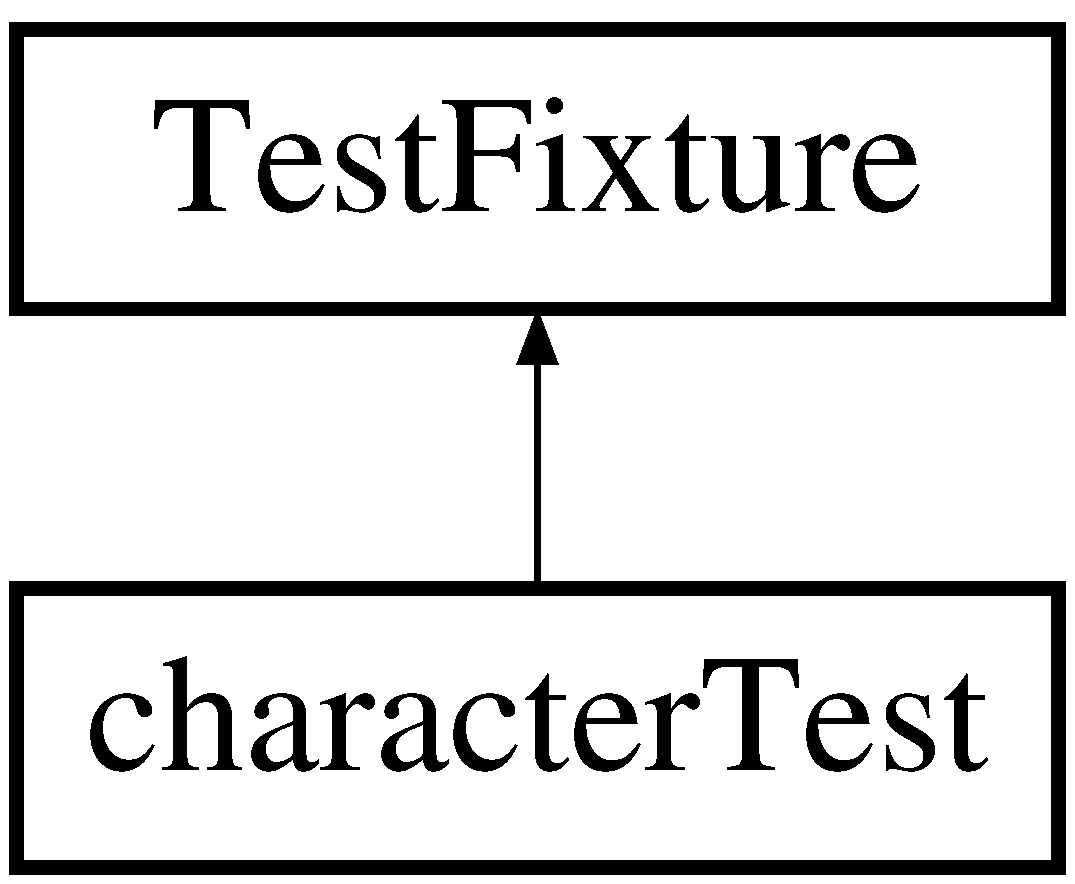
\includegraphics[height=2.000000cm]{classcharacter_test}
\end{center}
\end{figure}
\subsection*{Public Member Functions}
\begin{DoxyCompactItemize}
\item 
\hypertarget{classcharacter_test_ae910ab7281d7742a369b6d0f2e41eb7a}{}\label{classcharacter_test_ae910ab7281d7742a369b6d0f2e41eb7a} 
void {\bfseries set\+Up} (void)
\item 
\hypertarget{classcharacter_test_a3edc2253bc653272aabb62a3caa5a6a0}{}\label{classcharacter_test_a3edc2253bc653272aabb62a3caa5a6a0} 
void {\bfseries tear\+Down} (void)
\end{DoxyCompactItemize}
\subsection*{Protected Member Functions}
\begin{DoxyCompactItemize}
\item 
void \hyperlink{classcharacter_test_a815882850aa0cf833ee91ac412cfd185}{test\+Attach\+Observer} (void)
\item 
void \hyperlink{classcharacter_test_a7afc2a1b8e1e2575d658877a86133e50}{test\+Detach\+Observer} (void)
\end{DoxyCompactItemize}


\subsection{Member Function Documentation}
\hypertarget{classcharacter_test_a815882850aa0cf833ee91ac412cfd185}{}\label{classcharacter_test_a815882850aa0cf833ee91ac412cfd185} 
\index{character\+Test@{character\+Test}!test\+Attach\+Observer@{test\+Attach\+Observer}}
\index{test\+Attach\+Observer@{test\+Attach\+Observer}!character\+Test@{character\+Test}}
\subsubsection{\texorpdfstring{test\+Attach\+Observer()}{testAttachObserver()}}
{\footnotesize\ttfamily void character\+Test\+::test\+Attach\+Observer (\begin{DoxyParamCaption}\item[{void}]{ }\end{DoxyParamCaption})\hspace{0.3cm}{\ttfamily [protected]}}

Tests if an observer, once attached to a character, is contained in his observer set. \hypertarget{classcharacter_test_a7afc2a1b8e1e2575d658877a86133e50}{}\label{classcharacter_test_a7afc2a1b8e1e2575d658877a86133e50} 
\index{character\+Test@{character\+Test}!test\+Detach\+Observer@{test\+Detach\+Observer}}
\index{test\+Detach\+Observer@{test\+Detach\+Observer}!character\+Test@{character\+Test}}
\subsubsection{\texorpdfstring{test\+Detach\+Observer()}{testDetachObserver()}}
{\footnotesize\ttfamily void character\+Test\+::test\+Detach\+Observer (\begin{DoxyParamCaption}\item[{void}]{ }\end{DoxyParamCaption})\hspace{0.3cm}{\ttfamily [protected]}}

Tests if an observers, once detached from a subject, is no longer contained in its observers 

The documentation for this class was generated from the following file\+:\begin{DoxyCompactItemize}
\item 
test\+Qt/character\+Test.\+cpp\end{DoxyCompactItemize}

\hypertarget{classeditscreen}{}\section{editscreen Class Reference}
\label{classeditscreen}\index{editscreen@{editscreen}}
Inheritance diagram for editscreen\+:\begin{figure}[H]
\begin{center}
\leavevmode
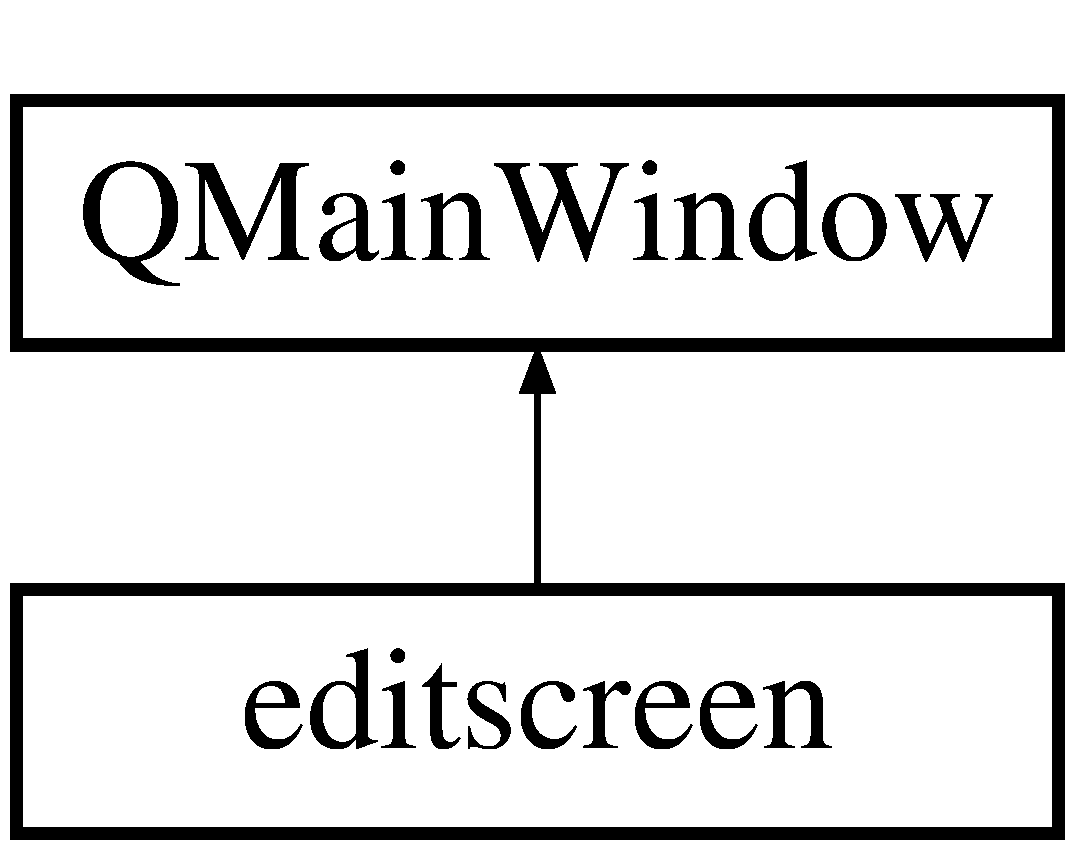
\includegraphics[height=2.000000cm]{classeditscreen}
\end{center}
\end{figure}
\subsection*{Public Slots}
\begin{DoxyCompactItemize}
\item 
\hypertarget{classeditscreen_ab87d295b62477e294f9436a2fc1087c0}{}\label{classeditscreen_ab87d295b62477e294f9436a2fc1087c0} 
void {\bfseries edit\+Map} ()
\item 
\hypertarget{classeditscreen_a054d2cef9dbc1bee9c4d29997eb7ef43}{}\label{classeditscreen_a054d2cef9dbc1bee9c4d29997eb7ef43} 
void {\bfseries open\+Map} ()
\item 
\hypertarget{classeditscreen_a2a62dec2be10d0aa5794d05429b7c2d5}{}\label{classeditscreen_a2a62dec2be10d0aa5794d05429b7c2d5} 
void {\bfseries new\+Map} ()
\end{DoxyCompactItemize}
\subsection*{Public Member Functions}
\begin{DoxyCompactItemize}
\item 
\hypertarget{classeditscreen_a7bc46501132eccf581229a731447167a}{}\label{classeditscreen_a7bc46501132eccf581229a731447167a} 
{\bfseries editscreen} (char n\mbox{[}$\,$\mbox{]})
\item 
\hypertarget{classeditscreen_a1be9e42a7542805e5f055f1a8a801e69}{}\label{classeditscreen_a1be9e42a7542805e5f055f1a8a801e69} 
bool {\bfseries get\+Window\+Open} ()
\end{DoxyCompactItemize}
\subsection*{Protected Member Functions}
\begin{DoxyCompactItemize}
\item 
\hypertarget{classeditscreen_a8ce99f3ff10200fe7d5d2686945a4257}{}\label{classeditscreen_a8ce99f3ff10200fe7d5d2686945a4257} 
void {\bfseries close\+Event} (Q\+Close\+Event $\ast$event)
\end{DoxyCompactItemize}


The documentation for this class was generated from the following files\+:\begin{DoxyCompactItemize}
\item 
test\+Qt/editscreen.\+h\item 
test\+Qt/editscreen.\+cpp\end{DoxyCompactItemize}

\hypertarget{class_grid_scene}{}\section{Grid\+Scene Class Reference}
\label{class_grid_scene}\index{Grid\+Scene@{Grid\+Scene}}
Inheritance diagram for Grid\+Scene\+:\begin{figure}[H]
\begin{center}
\leavevmode
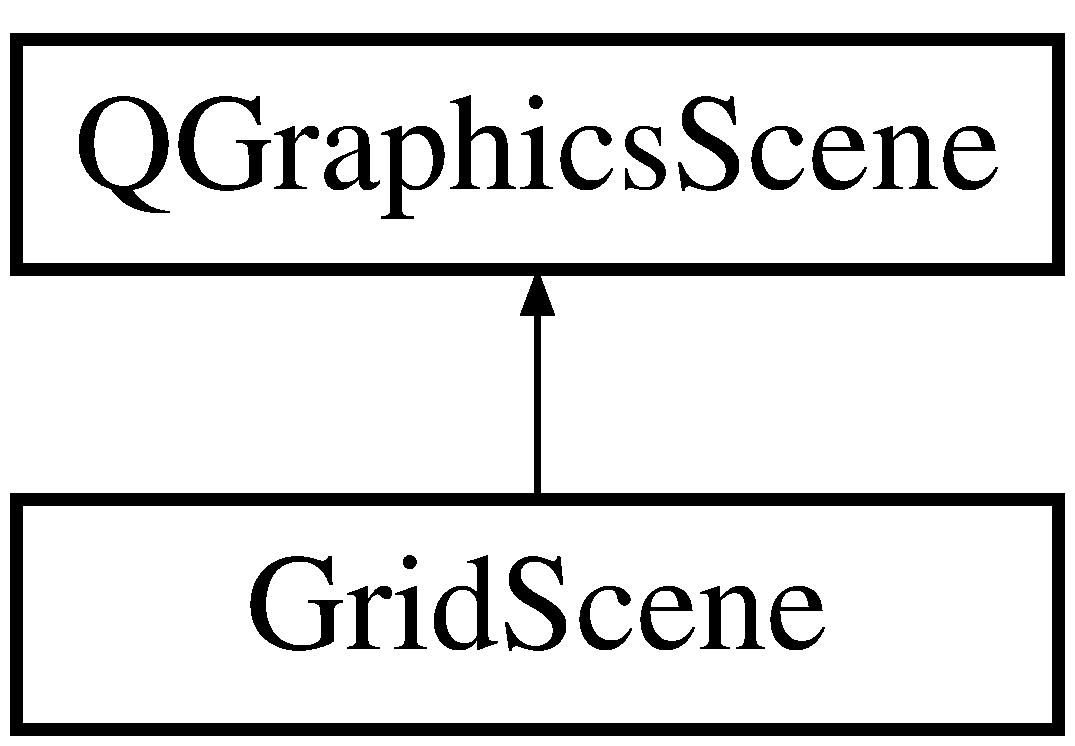
\includegraphics[height=2.000000cm]{class_grid_scene}
\end{center}
\end{figure}
\subsection*{Public Member Functions}
\begin{DoxyCompactItemize}
\item 
\hypertarget{class_grid_scene_a862e773b698ef7af7569c2c7fb8d30f4}{}\label{class_grid_scene_a862e773b698ef7af7569c2c7fb8d30f4} 
{\bfseries Grid\+Scene} (qreal x, qreal y, qreal w, qreal h)
\end{DoxyCompactItemize}
\subsection*{Protected Member Functions}
\begin{DoxyCompactItemize}
\item 
\hypertarget{class_grid_scene_a35c5f90bbf2f0ada9312b0097960c5ee}{}\label{class_grid_scene_a35c5f90bbf2f0ada9312b0097960c5ee} 
void {\bfseries draw\+Background} (Q\+Painter $\ast$painter, const Q\+RectF \&rect)
\end{DoxyCompactItemize}


The documentation for this class was generated from the following file\+:\begin{DoxyCompactItemize}
\item 
test\+Qt/Grid\+Scene.\+cpp\end{DoxyCompactItemize}

\hypertarget{classitem_container}{}\section{item\+Container Class Reference}
\label{classitem_container}\index{item\+Container@{item\+Container}}
\subsection*{Public Member Functions}
\begin{DoxyCompactItemize}
\item 
\hypertarget{classitem_container_a77987d5345c5e5d466a88a1df5f7d308}{}\label{classitem_container_a77987d5345c5e5d466a88a1df5f7d308} 
string {\bfseries get\+Type} (string file\+Path, int id)
\item 
\hypertarget{classitem_container_aa50daab99aacd53128603d38436f3546}{}\label{classitem_container_aa50daab99aacd53128603d38436f3546} 
string {\bfseries get\+Name} (string file\+Path, int id)
\item 
\hypertarget{classitem_container_a6292861f5177b32388322637a301aebd}{}\label{classitem_container_a6292861f5177b32388322637a301aebd} 
string {\bfseries get\+Enchantment} (string file\+Path, int id)
\item 
\hypertarget{classitem_container_a5542838aef955002f47bea0d8efdfb1c}{}\label{classitem_container_a5542838aef955002f47bea0d8efdfb1c} 
int {\bfseries get\+Bonus} (string file\+Path, int id)
\item 
\hypertarget{classitem_container_ad39d4af0d85626c18fd2db308aacb320}{}\label{classitem_container_ad39d4af0d85626c18fd2db308aacb320} 
string {\bfseries get\+Dice\+Or\+Grade} (string file\+Path, int id)
\item 
\hypertarget{classitem_container_a00613322b41793ea9805177c84aeb9fd}{}\label{classitem_container_a00613322b41793ea9805177c84aeb9fd} 
void {\bfseries add\+Item\+Backpack} (int id)
\item 
\hypertarget{classitem_container_a888fa7911cad5d08681f8528d4069c9b}{}\label{classitem_container_a888fa7911cad5d08681f8528d4069c9b} 
void {\bfseries remove\+Item\+Backpack} (int rnd)
\item 
\hypertarget{classitem_container_a5a9803d2e37c3454beec935d03a0672b}{}\label{classitem_container_a5a9803d2e37c3454beec935d03a0672b} 
void {\bfseries add\+Item\+Worn} (int id)
\item 
\hypertarget{classitem_container_af444b69ae3baeb89325574d764855d92}{}\label{classitem_container_af444b69ae3baeb89325574d764855d92} 
void {\bfseries remove\+Item\+Worn} (string item\+Type)
\end{DoxyCompactItemize}
\subsection*{Static Public Member Functions}
\begin{DoxyCompactItemize}
\item 
\hypertarget{classitem_container_a0351451d4184fb40c105d148d1e36887}{}\label{classitem_container_a0351451d4184fb40c105d148d1e36887} 
static string {\bfseries get\+All\+From\+File} (string file\+Path)
\end{DoxyCompactItemize}
\subsection*{Public Attributes}
\begin{DoxyCompactItemize}
\item 
\hypertarget{classitem_container_a0b93ed79558f99be509bc18448aec165}{}\label{classitem_container_a0b93ed79558f99be509bc18448aec165} 
string {\bfseries line}
\item 
\hypertarget{classitem_container_a6204c656f7f14a0778184434b1497d89}{}\label{classitem_container_a6204c656f7f14a0778184434b1497d89} 
int {\bfseries id}
\item 
\hypertarget{classitem_container_ae5891ff00750ee638fa2e115195df850}{}\label{classitem_container_ae5891ff00750ee638fa2e115195df850} 
string {\bfseries item}
\item 
\hypertarget{classitem_container_a81a860050cf20d1fd03cb78d16c294e7}{}\label{classitem_container_a81a860050cf20d1fd03cb78d16c294e7} 
string {\bfseries name}
\end{DoxyCompactItemize}


The documentation for this class was generated from the following files\+:\begin{DoxyCompactItemize}
\item 
test\+Qt/item\+Container.\+h\item 
test\+Qt/item\+Container.\+cpp\end{DoxyCompactItemize}

\hypertarget{classlogic}{}\section{logic Class Reference}
\label{classlogic}\index{logic@{logic}}
Inheritance diagram for logic\+:\begin{figure}[H]
\begin{center}
\leavevmode
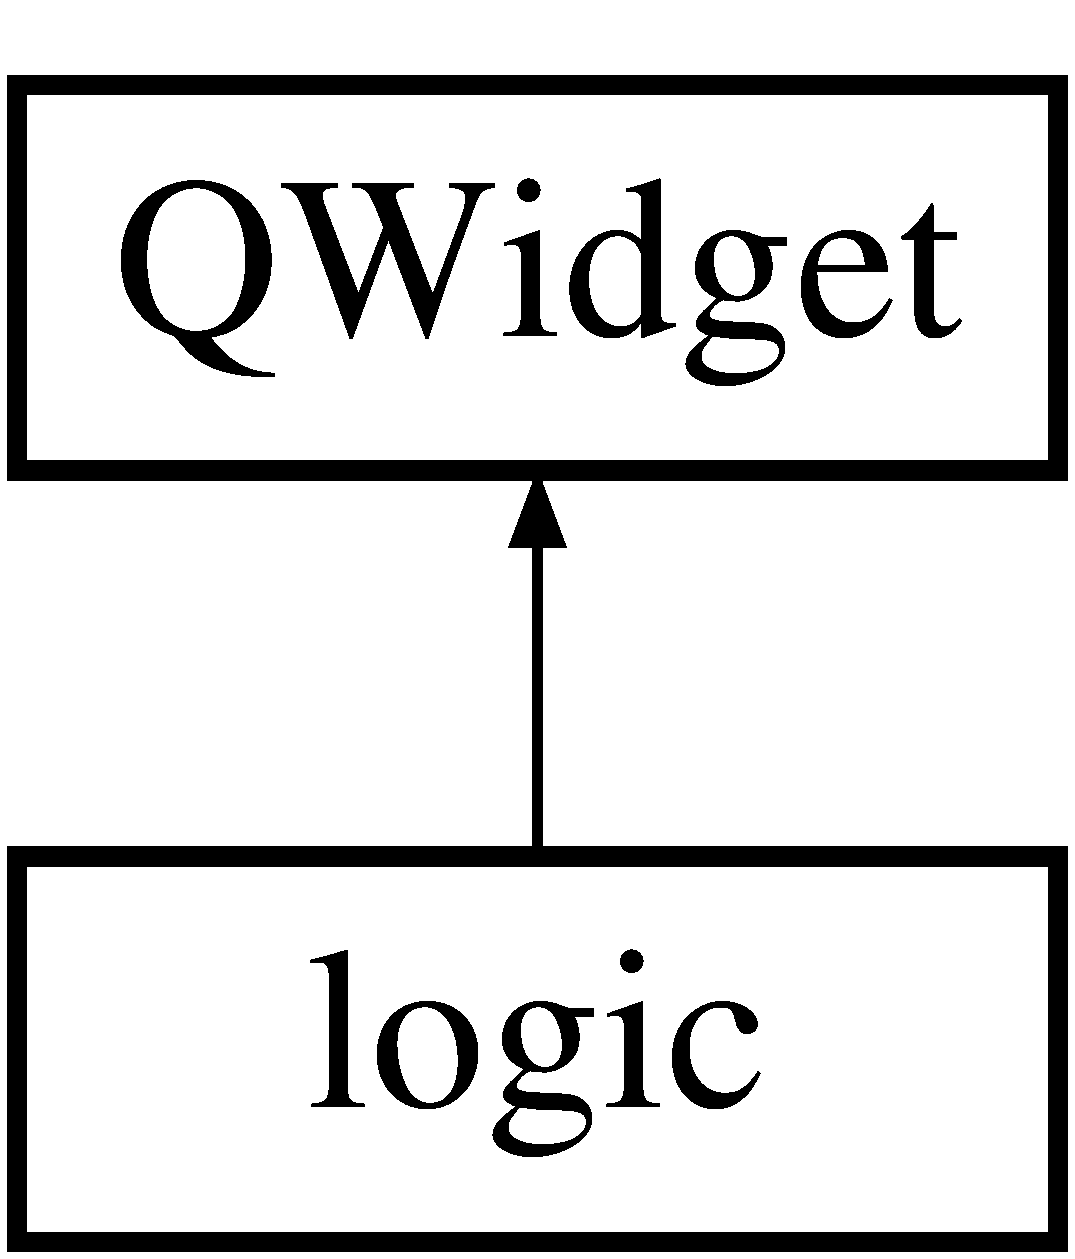
\includegraphics[height=2.000000cm]{classlogic}
\end{center}
\end{figure}
\subsection*{Public Member Functions}
\begin{DoxyCompactItemize}
\item 
\hypertarget{classlogic_afeb64b81f69e6d1f66421d9e49fab832}{}\label{classlogic_afeb64b81f69e6d1f66421d9e49fab832} 
{\bfseries logic} (Q\+Widget $\ast$parent=0)
\item 
\hypertarget{classlogic_af867500c17777425154268768a9eb463}{}\label{classlogic_af867500c17777425154268768a9eb463} 
void {\bfseries initialize} (int w, int h)
\item 
\hypertarget{classlogic_a30e87e24b2850a02828f9c11291eb001}{}\label{classlogic_a30e87e24b2850a02828f9c11291eb001} 
void {\bfseries set\+Resolution} (int res)
\item 
\hypertarget{classlogic_ad3a599ff9c7f5a3e84379f0a121010fc}{}\label{classlogic_ad3a599ff9c7f5a3e84379f0a121010fc} 
void {\bfseries load\+Map} (string filename)
\item 
\hypertarget{classlogic_a28ab425885566a86b0700fdeeacc9255}{}\label{classlogic_a28ab425885566a86b0700fdeeacc9255} 
int {\bfseries get\+Width} ()
\item 
\hypertarget{classlogic_afc7a47dc48d48f258e8b5a1ce36b1d7f}{}\label{classlogic_afc7a47dc48d48f258e8b5a1ce36b1d7f} 
int {\bfseries get\+Height} ()
\item 
\hypertarget{classlogic_a01b2dc69b06a0de6483c5321fc5cd49d}{}\label{classlogic_a01b2dc69b06a0de6483c5321fc5cd49d} 
bool {\bfseries get\+Window\+Open} ()
\end{DoxyCompactItemize}
\subsection*{Protected Member Functions}
\begin{DoxyCompactItemize}
\item 
\hypertarget{classlogic_a6a12964d5c28d729acba713550bdba43}{}\label{classlogic_a6a12964d5c28d729acba713550bdba43} 
void {\bfseries mouse\+Press\+Event} (Q\+Mouse\+Event $\ast$event) Q\+\_\+\+D\+E\+C\+L\+\_\+\+O\+V\+E\+R\+R\+I\+DE
\item 
\hypertarget{classlogic_acb187bd764b1c2478c9a0792268c849e}{}\label{classlogic_acb187bd764b1c2478c9a0792268c849e} 
void {\bfseries paint\+Event} (Q\+Paint\+Event $\ast$event) Q\+\_\+\+D\+E\+C\+L\+\_\+\+O\+V\+E\+R\+R\+I\+DE
\item 
\hypertarget{classlogic_a9d4eb2785a9b5ba90667ea917af0214f}{}\label{classlogic_a9d4eb2785a9b5ba90667ea917af0214f} 
void {\bfseries resize\+Event} (Q\+Resize\+Event $\ast$event) Q\+\_\+\+D\+E\+C\+L\+\_\+\+O\+V\+E\+R\+R\+I\+DE
\item 
\hypertarget{classlogic_aee48c6aa61703aa595a25e99ea8f18e6}{}\label{classlogic_aee48c6aa61703aa595a25e99ea8f18e6} 
void {\bfseries leave\+Event} (Q\+Event $\ast$event) Q\+\_\+\+D\+E\+C\+L\+\_\+\+O\+V\+E\+R\+R\+I\+DE
\end{DoxyCompactItemize}


The documentation for this class was generated from the following files\+:\begin{DoxyCompactItemize}
\item 
test\+Qt/logic.\+h\item 
test\+Qt/logic.\+cpp\end{DoxyCompactItemize}

\hypertarget{class_map_screen}{}\section{Map\+Screen Class Reference}
\label{class_map_screen}\index{Map\+Screen@{Map\+Screen}}
\subsection*{Public Member Functions}
\begin{DoxyCompactItemize}
\item 
\hypertarget{class_map_screen_a7ec8d9c66912e402e57bfdd7778a5b13}{}\label{class_map_screen_a7ec8d9c66912e402e57bfdd7778a5b13} 
void {\bfseries init\+Map} (int x, int y)
\item 
\hypertarget{class_map_screen_af90b7b04c0534eca6587e27ec20c116e}{}\label{class_map_screen_af90b7b04c0534eca6587e27ec20c116e} 
int {\bfseries get\+CurrentX} ()
\item 
\hypertarget{class_map_screen_ad351362c23dc6d214ef04656ab82746a}{}\label{class_map_screen_ad351362c23dc6d214ef04656ab82746a} 
int {\bfseries get\+CurrentY} ()
\item 
\hypertarget{class_map_screen_a172790eebb34a12a54902779185f3737}{}\label{class_map_screen_a172790eebb34a12a54902779185f3737} 
int {\bfseries get\+StartX} ()
\item 
\hypertarget{class_map_screen_a4b81f948186249a2a03e5b18d3b8a45f}{}\label{class_map_screen_a4b81f948186249a2a03e5b18d3b8a45f} 
int {\bfseries get\+StartY} ()
\item 
\hypertarget{class_map_screen_a4809056226797d7dcdc7989e30412abb}{}\label{class_map_screen_a4809056226797d7dcdc7989e30412abb} 
int {\bfseries get\+EndX} ()
\item 
\hypertarget{class_map_screen_ab61eb74b352f9faaf258cbf51afd99d6}{}\label{class_map_screen_ab61eb74b352f9faaf258cbf51afd99d6} 
int {\bfseries get\+EndY} ()
\item 
\hypertarget{class_map_screen_a65f5581be2db9d0493df849c2c99b170}{}\label{class_map_screen_a65f5581be2db9d0493df849c2c99b170} 
void {\bfseries set\+StartX} (int x)
\item 
\hypertarget{class_map_screen_afbaa726dc7180c94da7eeb3214e8e8f0}{}\label{class_map_screen_afbaa726dc7180c94da7eeb3214e8e8f0} 
void {\bfseries set\+StartY} (int y)
\item 
\hypertarget{class_map_screen_a96ef52b100fba7b34f3b3914a9f2b92a}{}\label{class_map_screen_a96ef52b100fba7b34f3b3914a9f2b92a} 
void {\bfseries set\+EndX} (int x)
\item 
\hypertarget{class_map_screen_a442a043c7ef47c4fe82d58deef54cb65}{}\label{class_map_screen_a442a043c7ef47c4fe82d58deef54cb65} 
void {\bfseries set\+EndY} (int y)
\item 
\hypertarget{class_map_screen_a86de80d62cbd8c0acea2ed33998c396b}{}\label{class_map_screen_a86de80d62cbd8c0acea2ed33998c396b} 
bool {\bfseries is\+Passable} ()
\item 
\hypertarget{class_map_screen_acf34be7d25ac28d475d748b22a952df0}{}\label{class_map_screen_acf34be7d25ac28d475d748b22a952df0} 
bool {\bfseries is\+Passable} (int x, int y)
\item 
\hypertarget{class_map_screen_aa73a3953e6698f7ea827c3c2c1c5ec35}{}\label{class_map_screen_aa73a3953e6698f7ea827c3c2c1c5ec35} 
bool {\bfseries is\+Occupied} (int x, int y)
\item 
\hypertarget{class_map_screen_a4583f04d132ce365ff609a4c2f204afb}{}\label{class_map_screen_a4583f04d132ce365ff609a4c2f204afb} 
void {\bfseries set\+Occupied} (int x, int y, bool pass)
\item 
\hypertarget{class_map_screen_a32c18aa83af5af7fab6e07f90869a458}{}\label{class_map_screen_a32c18aa83af5af7fab6e07f90869a458} 
void {\bfseries set\+Passable} (int x, int y, bool pass)
\item 
\hypertarget{class_map_screen_a2a108e5d1fbe259c2027ef37e5940481}{}\label{class_map_screen_a2a108e5d1fbe259c2027ef37e5940481} 
int {\bfseries get\+Number\+Of\+Distinct\+N\+P\+Cs} ()
\item 
\hypertarget{class_map_screen_aee2e1392794eac96986bacbbe740cabb}{}\label{class_map_screen_aee2e1392794eac96986bacbbe740cabb} 
int {\bfseries get\+Number\+Of\+N\+P\+Cs} ()
\item 
\hypertarget{class_map_screen_a06feaaa9d453707bbf543f5794cf22c7}{}\label{class_map_screen_a06feaaa9d453707bbf543f5794cf22c7} 
bool {\bfseries check\+Exit} ()
\item 
\hypertarget{class_map_screen_a91dff80abc0d95a877d6a6ba289f4924}{}\label{class_map_screen_a91dff80abc0d95a877d6a6ba289f4924} 
int {\bfseries get\+MaxX} ()
\item 
\hypertarget{class_map_screen_a078b380601f48e4fefc83420f673d0f6}{}\label{class_map_screen_a078b380601f48e4fefc83420f673d0f6} 
int {\bfseries get\+MaxY} ()
\item 
\hypertarget{class_map_screen_a28cdac5ec3963d90af6adab6e12c7226}{}\label{class_map_screen_a28cdac5ec3963d90af6adab6e12c7226} 
void {\bfseries save\+To\+File} (string f\+Name)
\item 
\hypertarget{class_map_screen_a7c3d724b7df47905c2b6310fa5ea894d}{}\label{class_map_screen_a7c3d724b7df47905c2b6310fa5ea894d} 
void {\bfseries load\+From\+File} (string filename)
\item 
\hypertarget{class_map_screen_a6314d018f5cd93f6a7c5cca2c96cd9c0}{}\label{class_map_screen_a6314d018f5cd93f6a7c5cca2c96cd9c0} 
void {\bfseries load\+N\+P\+Cs} ()
\item 
\hypertarget{class_map_screen_a9319425b52da0c0c1860fdf123724fa5}{}\label{class_map_screen_a9319425b52da0c0c1860fdf123724fa5} 
bool {\bfseries add\+N\+PC} (int id, int x\+Pos, int y\+Pos)
\item 
\hypertarget{class_map_screen_a47a88c4b46017ac1754f6208516e4c24}{}\label{class_map_screen_a47a88c4b46017ac1754f6208516e4c24} 
void {\bfseries remove\+N\+PC} (int x\+Pos, int y\+Pos)
\end{DoxyCompactItemize}
\subsection*{Public Attributes}
\begin{DoxyCompactItemize}
\item 
\hypertarget{class_map_screen_af3db400915544bc7a680711ee16a46f7}{}\label{class_map_screen_af3db400915544bc7a680711ee16a46f7} 
\hyperlink{classcharacter}{character} {\bfseries character\+Table} \mbox{[}10\mbox{]}
\item 
\hypertarget{class_map_screen_aba782e08ff8c1d02476b0a9e22cc1445}{}\label{class_map_screen_aba782e08ff8c1d02476b0a9e22cc1445} 
\hyperlink{classcharacter}{character} {\bfseries character\+Entities} \mbox{[}100\mbox{]}
\end{DoxyCompactItemize}


The documentation for this class was generated from the following files\+:\begin{DoxyCompactItemize}
\item 
test\+Qt/Map\+Screen.\+h\item 
test\+Qt/Map\+Screen.\+cpp\end{DoxyCompactItemize}

\hypertarget{classobserver}{}\section{observer Class Reference}
\label{classobserver}\index{observer@{observer}}


{\ttfamily \#include $<$observer.\+h$>$}

Inheritance diagram for observer\+:\begin{figure}[H]
\begin{center}
\leavevmode
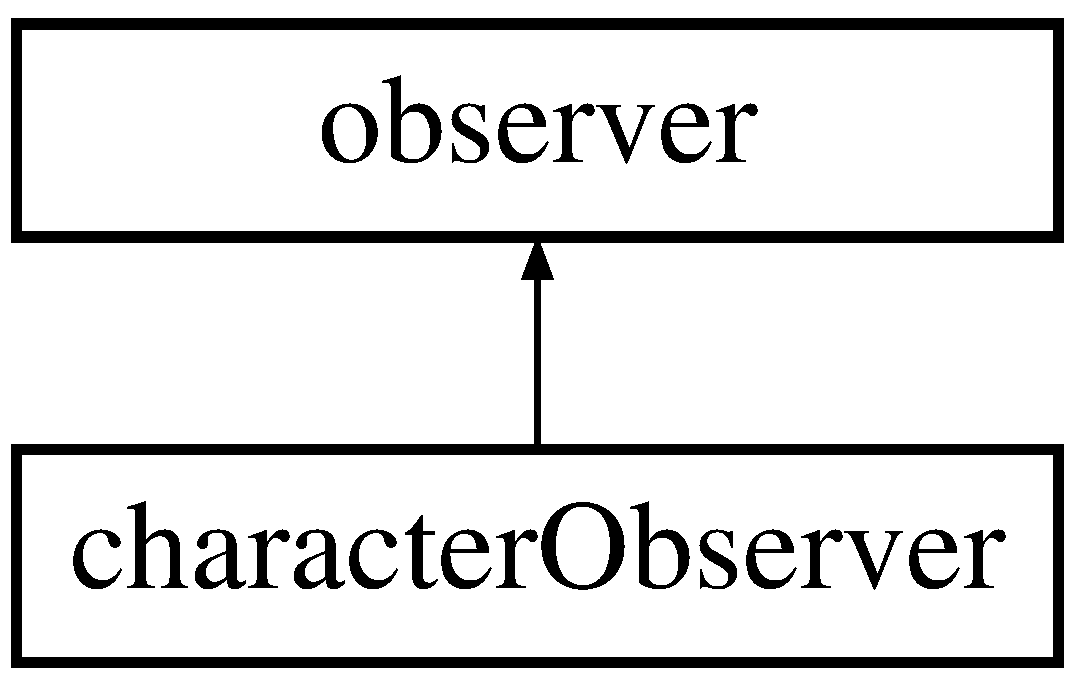
\includegraphics[height=2.000000cm]{classobserver}
\end{center}
\end{figure}
\subsection*{Public Member Functions}
\begin{DoxyCompactItemize}
\item 
\hypertarget{classobserver_a598c062264bb62e6e74a5b187c7bcfa7}{}\label{classobserver_a598c062264bb62e6e74a5b187c7bcfa7} 
virtual void {\bfseries notify} ()=0
\end{DoxyCompactItemize}


\subsection{Detailed Description}
Abstract class for implementation of observer pattern 

The documentation for this class was generated from the following files\+:\begin{DoxyCompactItemize}
\item 
test\+Qt/observer.\+h\item 
test\+Qt/observer.\+cpp\end{DoxyCompactItemize}

\hypertarget{class_q___debug_stream}{}\section{Q\+\_\+\+Debug\+Stream Class Reference}
\label{class_q___debug_stream}\index{Q\+\_\+\+Debug\+Stream@{Q\+\_\+\+Debug\+Stream}}
Inheritance diagram for Q\+\_\+\+Debug\+Stream\+:\begin{figure}[H]
\begin{center}
\leavevmode
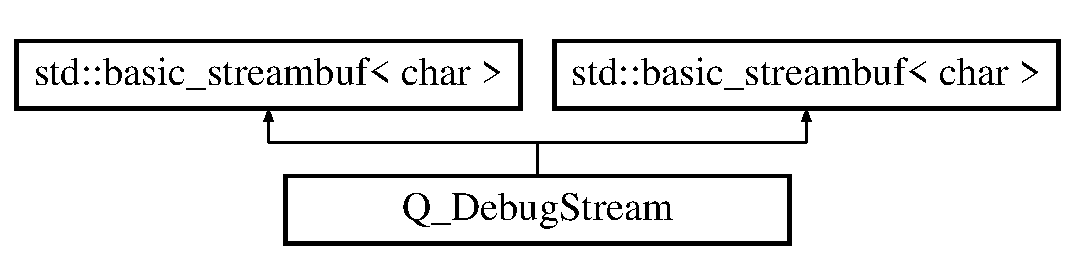
\includegraphics[height=2.000000cm]{class_q___debug_stream}
\end{center}
\end{figure}
\subsection*{Public Member Functions}
\begin{DoxyCompactItemize}
\item 
\hypertarget{class_q___debug_stream_a34eaae6399620da13cac980c4b10bea4}{}\label{class_q___debug_stream_a34eaae6399620da13cac980c4b10bea4} 
{\bfseries Q\+\_\+\+Debug\+Stream} (std\+::ostream \&stream)
\item 
\hypertarget{class_q___debug_stream_a34eaae6399620da13cac980c4b10bea4}{}\label{class_q___debug_stream_a34eaae6399620da13cac980c4b10bea4} 
{\bfseries Q\+\_\+\+Debug\+Stream} (std\+::ostream \&stream)
\end{DoxyCompactItemize}
\subsection*{Protected Member Functions}
\begin{DoxyCompactItemize}
\item 
\hypertarget{class_q___debug_stream_aeface8c7f01a29d55142c36ff7600d29}{}\label{class_q___debug_stream_aeface8c7f01a29d55142c36ff7600d29} 
virtual int\+\_\+type {\bfseries overflow} (int\+\_\+type v)
\item 
\hypertarget{class_q___debug_stream_a46def7b89b4f656eed40a6b3f9f76324}{}\label{class_q___debug_stream_a46def7b89b4f656eed40a6b3f9f76324} 
virtual std\+::streamsize {\bfseries xsputn} (const char $\ast$p, std\+::streamsize n)
\item 
\hypertarget{class_q___debug_stream_aeface8c7f01a29d55142c36ff7600d29}{}\label{class_q___debug_stream_aeface8c7f01a29d55142c36ff7600d29} 
virtual int\+\_\+type {\bfseries overflow} (int\+\_\+type v)
\item 
\hypertarget{class_q___debug_stream_a46def7b89b4f656eed40a6b3f9f76324}{}\label{class_q___debug_stream_a46def7b89b4f656eed40a6b3f9f76324} 
virtual std\+::streamsize {\bfseries xsputn} (const char $\ast$p, std\+::streamsize n)
\end{DoxyCompactItemize}


The documentation for this class was generated from the following files\+:\begin{DoxyCompactItemize}
\item 
test\+Qt/Q\+\_\+\+Debug\+Stream.\+cpp\item 
test\+Qt/Q\+\_\+\+Debug\+Stream.\+h\end{DoxyCompactItemize}

\hypertarget{struct_search}{}\section{Search Struct Reference}
\label{struct_search}\index{Search@{Search}}
\subsection*{Public Attributes}
\begin{DoxyCompactItemize}
\item 
\hypertarget{struct_search_a87992fbf082d7d1bb6095fc645df7337}{}\label{struct_search_a87992fbf082d7d1bb6095fc645df7337} 
bool {\bfseries north\+Searched} = false
\item 
\hypertarget{struct_search_a258093c1b694f7be1cd3bd96f9e08f5c}{}\label{struct_search_a258093c1b694f7be1cd3bd96f9e08f5c} 
bool {\bfseries east\+Searched} = false
\item 
\hypertarget{struct_search_ad00469a5393f6d7627042da1d31fc56a}{}\label{struct_search_ad00469a5393f6d7627042da1d31fc56a} 
bool {\bfseries south\+Searched} = false
\item 
\hypertarget{struct_search_a14328c1d137d9608f6382309a47676a4}{}\label{struct_search_a14328c1d137d9608f6382309a47676a4} 
bool {\bfseries west\+Searched} = false
\item 
\hypertarget{struct_search_aecab176131f37e3751f5dfb5d62b1207}{}\label{struct_search_aecab176131f37e3751f5dfb5d62b1207} 
string {\bfseries space\+Came\+From} = \char`\"{}\char`\"{}
\item 
\hypertarget{struct_search_aac7791842d53dca0b23f4bf23fd2796d}{}\label{struct_search_aac7791842d53dca0b23f4bf23fd2796d} 
bool {\bfseries explored} = false
\item 
\hypertarget{struct_search_a37e87cd6ae0c7e02715e4cdd57af2015}{}\label{struct_search_a37e87cd6ae0c7e02715e4cdd57af2015} 
bool {\bfseries dead\+End} = false
\end{DoxyCompactItemize}


The documentation for this struct was generated from the following file\+:\begin{DoxyCompactItemize}
\item 
test\+Qt/Map\+Screen.\+cpp\end{DoxyCompactItemize}

\hypertarget{struct_space}{}\section{Space Struct Reference}
\label{struct_space}\index{Space@{Space}}
\subsection*{Public Attributes}
\begin{DoxyCompactItemize}
\item 
\hypertarget{struct_space_a9b97b8498860f8eaf1e069ee8359c82e}{}\label{struct_space_a9b97b8498860f8eaf1e069ee8359c82e} 
bool {\bfseries passable} = true
\item 
\hypertarget{struct_space_a4a32796e863087ca621c8d82f5a1a58e}{}\label{struct_space_a4a32796e863087ca621c8d82f5a1a58e} 
bool {\bfseries occupied} = false
\end{DoxyCompactItemize}


The documentation for this struct was generated from the following file\+:\begin{DoxyCompactItemize}
\item 
test\+Qt/Map\+Screen.\+h\end{DoxyCompactItemize}

\hypertarget{classtest_qt}{}\section{test\+Qt Class Reference}
\label{classtest_qt}\index{test\+Qt@{test\+Qt}}
Inheritance diagram for test\+Qt\+:\begin{figure}[H]
\begin{center}
\leavevmode
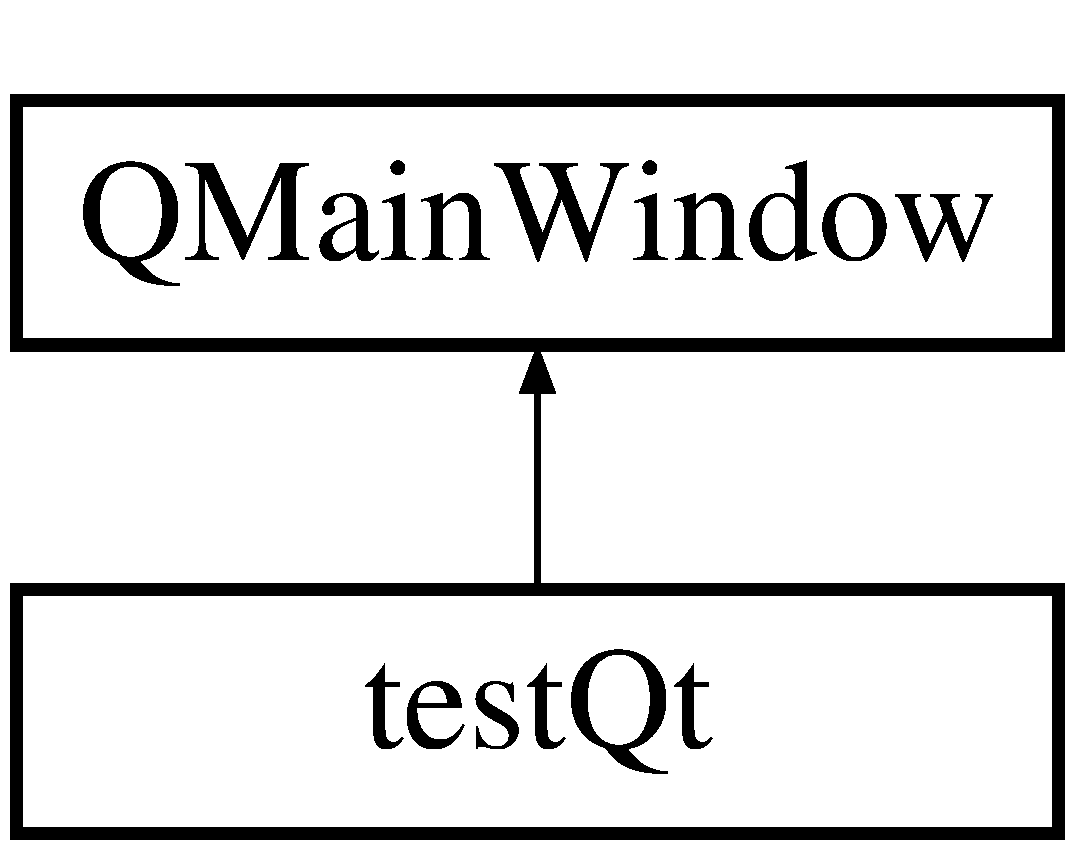
\includegraphics[height=2.000000cm]{classtest_qt}
\end{center}
\end{figure}
\subsection*{Public Member Functions}
\begin{DoxyCompactItemize}
\item 
\hypertarget{classtest_qt_a6ea0c0f87dde2bf02654cbccb5c2223b}{}\label{classtest_qt_a6ea0c0f87dde2bf02654cbccb5c2223b} 
{\bfseries test\+Qt} (Q\+Widget $\ast$parent=0)
\end{DoxyCompactItemize}


The documentation for this class was generated from the following files\+:\begin{DoxyCompactItemize}
\item 
test\+Qt/testqt.\+h\item 
test\+Qt/testqt.\+cpp\end{DoxyCompactItemize}

%--- End generated contents ---

% Index
\backmatter
\newpage
\phantomsection
\clearemptydoublepage
\addcontentsline{toc}{chapter}{Index}
\printindex

\end{document}
